\documentclass[tikz]{standalone}

\usepackage{amsmath}
\usepackage{unicode-math}
\usepackage{mathtools}
\usepackage{derivative}

\setmainfont{Stix Two Text}
\setmathfont{Stix Two Math}

\usetikzlibrary{arrows.meta,fit,positioning}

\renewcommand{\familydefault}{\sfdefault}

% prefix equation numbers with section number
\numberwithin{equation}{section}

\DeclarePairedDelimiter{\ceil}{\lceil}{\rceil}
\DeclarePairedDelimiter{\floor}{\lfloor}{\rfloor}
\DeclarePairedDelimiter{\abs}{\lvert}{\rvert}
\DeclarePairedDelimiter{\norm}{\lVert}{\rVert}
\DeclarePairedDelimiter{\bra}{\langle}{\rvert}
\DeclarePairedDelimiter{\ket}{\lvert}{\rangle}
\DeclarePairedDelimiter{\expval}{\langle}{\rangle}
\DeclarePairedDelimiter{\norder}{\mathcolon}{\mathcolon}
\DeclarePairedDelimiter{\anorder}{\typecolon}{\typecolon}
	
\newcommand{\laplace}{\mbfnabla^2}
\newcommand{\trans}{{\scriptscriptstyle\mathsf{T}}}

\newcommand{\vdot}{\cdot}
\newcommand{\vcross}{\vectimes}
\newcommand{\vb}[1]{\symbfup{#1}}
\newcommand{\vu}[1]{\hat{\vb{#1}}}
\newcommand*\dd[2][\relax]{\mathop{\ifx\relax#1\odif{#2}\else \odif[order={#1}]{#2}\fi\,}}

\newcommand{\vacuum}{\ket*{\vb{0}}}

\DeclareMathOperator{\trace}{Tr}
\DeclareMathOperator{\sinc}{sinc}

\AtBeginDocument{
	\let\Re\relax
	\let\Im\relax
	\DeclareMathOperator{\Re}{Re}
	\DeclareMathOperator{\Im}{Im}

	\renewcommand{\div}{\mathop{\mbfnabla\vdot}}
	\newcommand{\curl}{\mathop{\mbfnabla\vectimes}}
}

\DeclarePairedDelimiterX{\comm}[2]{[}{]}{#1,#2}

\DeclarePairedDelimiterX{\braket}[2]{\langle}{\rangle}{#1\delimsize\vert#2}
\DeclarePairedDelimiterX{\ketbra}[1]{\lvert}{\rvert}{#1\rangle\delimsize\langle#1}



\usepgfplotslibrary{groupplots}

\begin{document}
	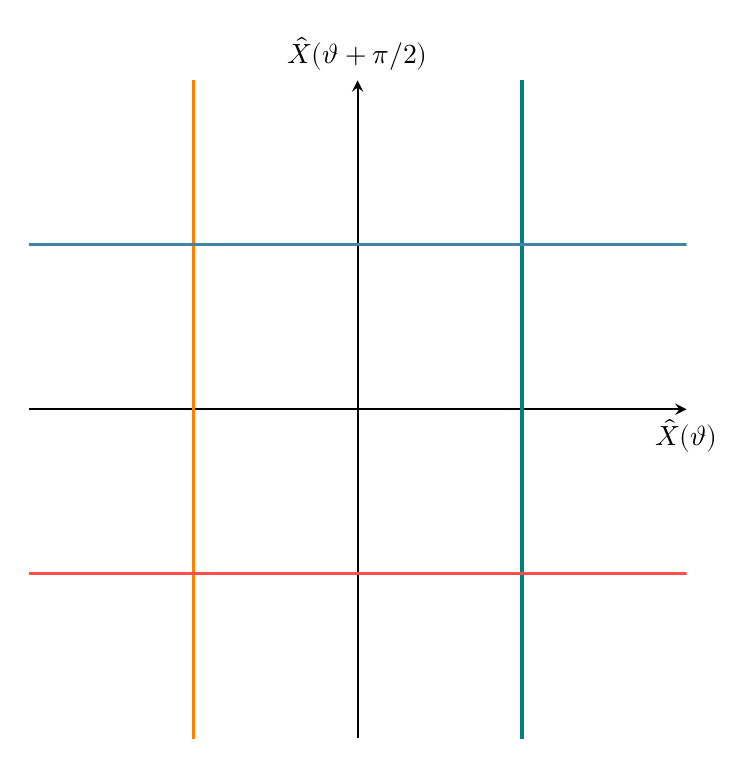
\begin{tikzpicture}
		\begin{axis}[
			width=0.95\linewidth,
			axis lines=center,
			axis equal image,
			axis line style=thick,
			xlabel={$\hat{X}(\vartheta)$},
			ylabel={$\hat{X}(\vartheta+\pi/2)$},
			ticks=none,
			xmin=-2,
			xmax=+2,
			ymin=-2,
			ymax=+2,
			axis line style={thick},
			x label style={
				at={(axis description cs:1,0.5)},
				anchor=north,
			},
			y label style={
				at={(axis description cs:0.5,1)},
				anchor=south,
			},
			cycle list name=exotic,
				legend style={
					at={(axis cs: 4,0)},
					anchor=east,
					inner sep=5,
					outer sep=10,
				},
			legend cell align={left},
		]
			\addplot+[very thick, no markers] coordinates {(1,-4) (1,0) (1,4)};
%			\addlegendentry{$\ket{+x,\vartheta}$};
			\addplot+[very thick, no markers] coordinates {(-1,-4) (-1,0) (-1,4)};
%			\addlegendentry{$\ket{-x,\vartheta}$};
			\addplot+[very thick, no markers] coordinates {(-4,1) (0,1) (4,1)};
%			\addlegendentry{$\ket{+x,\vartheta+\pi/2}$};
			\addplot+[very thick, no markers] coordinates {(-4,-1) (0,-1) (4,-1)};
%			\addlegendentry{$\ket{-x,\vartheta+\pi/2}$};
		\end{axis}
	\end{tikzpicture}
\end{document}